\section{Bruit 5G}

Lorsqu'un appareil émet sur le spectre de la 5G, il devient particulièrement sensible aux interférences électromagnétiques voire figure \ref{fig:bruit-5g}. Cela peut fausser les mesures réalisées à proximité, car les signaux émis peuvent perturber les instruments de mesure. Il est donc essentiel d'éloigner les appareils émettant sur ces fréquences afin de garantir la fiabilité et la précision des résultats obtenus.
\begin{figure}[H]
    \centering
    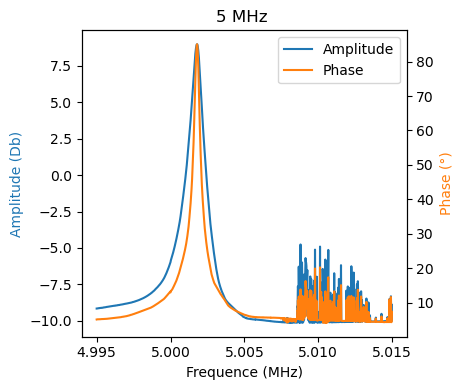
\includegraphics[width=0.8\textwidth]{assets/figures/bruit5G.png}
    \caption{Illustration du bruit 5G}
    \label{fig:bruit-5g}
\end{figure}
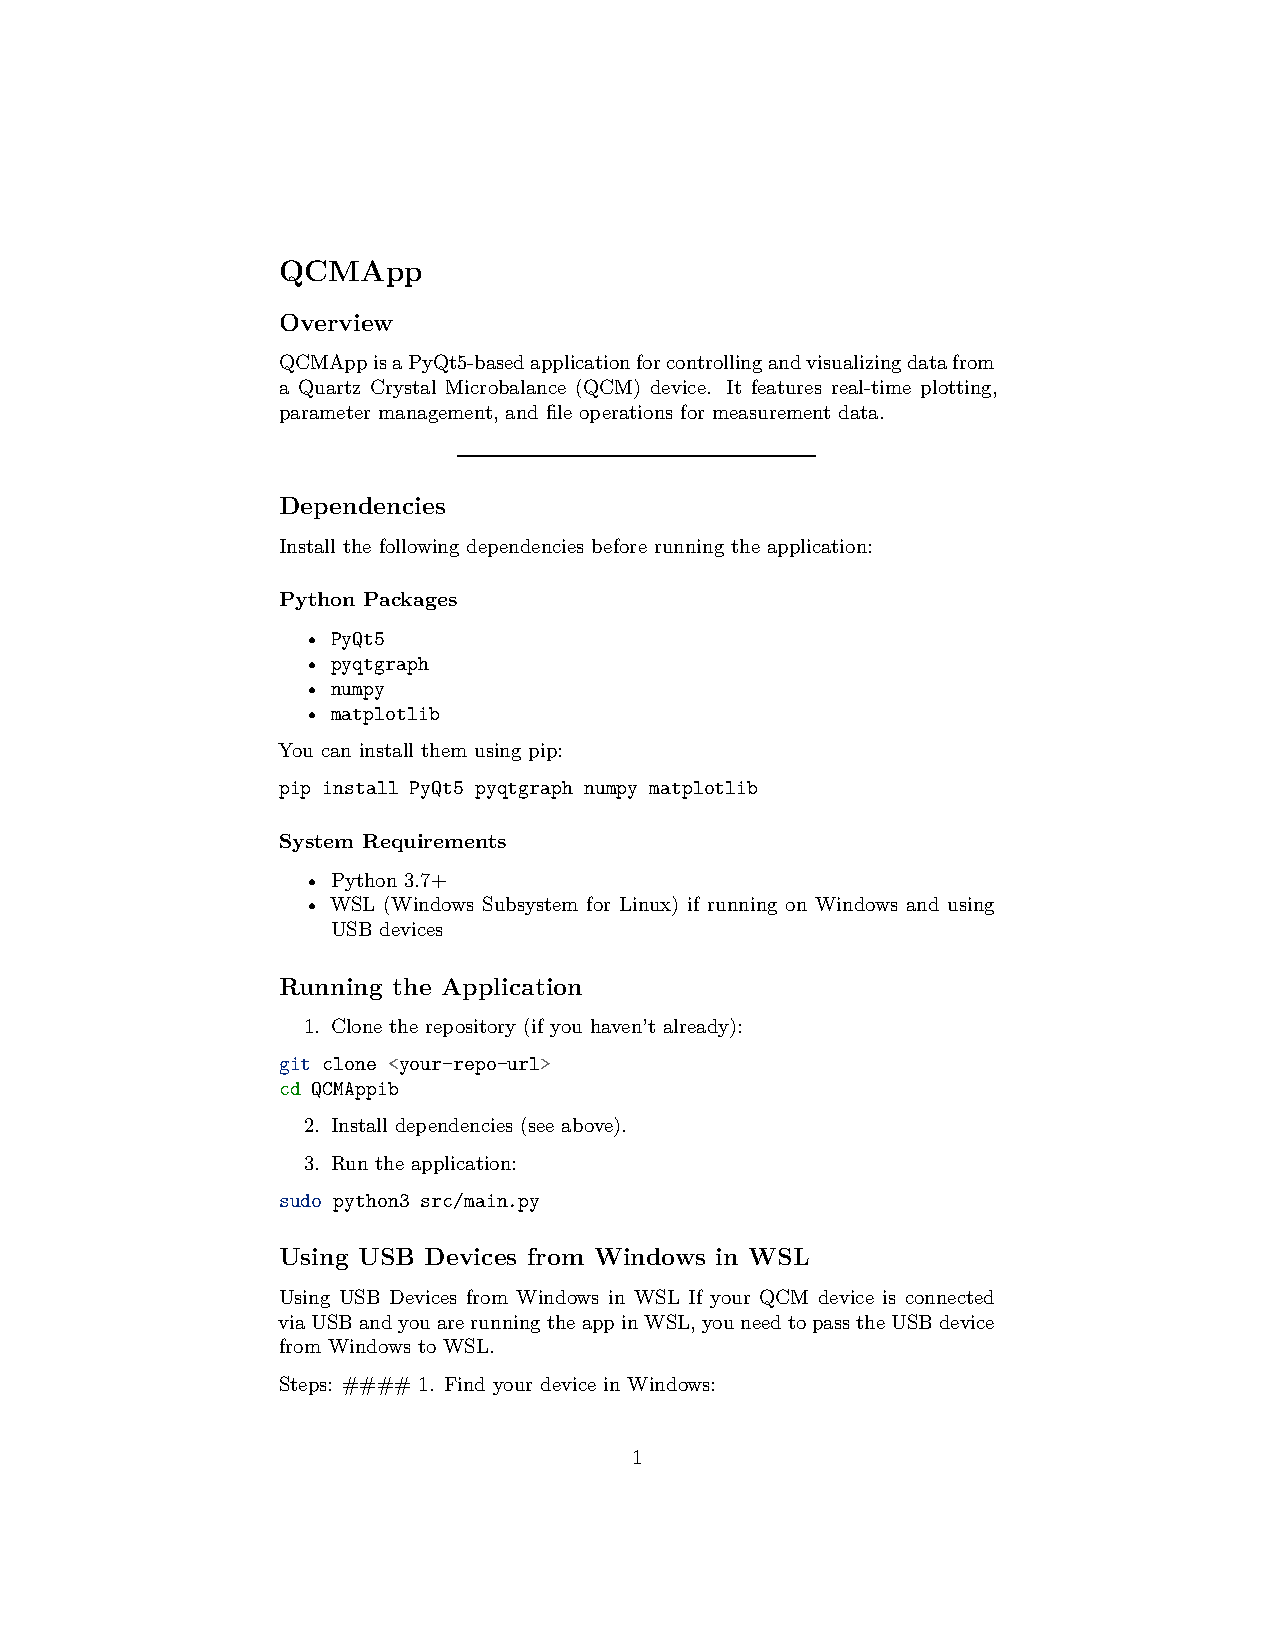
\includepdf[pages=-]{assets/readme.pdf}